\documentclass[10pt]{article}

\usepackage[a4paper, margin=2cm]{geometry}
\usepackage[T1]{fontenc}
\usepackage{lmodern}
\usepackage{microtype}
\usepackage{graphicx}
\usepackage{booktabs}
\usepackage{amsmath}
\usepackage{caption}
\usepackage{subcaption}
\usepackage{enumitem}
\usepackage[hidelinks]{hyperref}

\graphicspath{{figures/}{../outputs/figures/}}
\captionsetup{font=small, labelfont=bf}
\setlist{itemsep=1pt, topsep=3pt}
\setlength{\parskip}{3pt}

\title{\vspace{-1.6cm}\textbf{Classifying Countries by Human Development Index\\from Socioeconomic Indicators}\vspace{-0.3cm}}
\author{Vivaan Singhania\\\small 25B2136 \and Shivam Kushwaha\\\small 25B2146 \and Tanush Chilakwad\\\small 25B2208}
\date{\vspace{-0.3cm}\small DS203 Course Project\vspace{-0.4cm}}

\begin{document}
\maketitle

% =====================================================================
\section{Introduction}

The Human Development Index (HDI) published by the UNDP summarises a country's development in three
dimensions: a long and healthy life, education, and standard of living. It is a widely used yardstick, but it
is published with a delay and depends on data (life expectancy, schooling, national income) that is not always
available or up to date. Economic and infrastructure indicators such as internet use, access to electricity or the
structure of the economy are collected more widely by the World Bank.

In this project we ask whether these more commonly available indicators are enough to place a country in the
right HDI category, and which of them carry the most information. We frame it as a three-class problem built
from the 2023 HDI score: \textbf{Low} (HDI $<0.550$), \textbf{Medium/High} ($0.550\le\text{HDI}<0.800$) and
\textbf{Very High} (HDI $\ge0.800$). This grouping was defined for the project and is not an official UNDP
classification (UNDP uses four categories).

We compare a majority-class baseline, multinomial logistic regression, a decision tree and a random forest. We
also study how missing data should be handled, whether PCA keeps the useful information, and how much the
categorical features (region and the dominant economic sector) add on top of the numerical indicators. Because
the data describes countries rather than individuals, every result should be read as an association, not a causal
effect.

% =====================================================================
\section{Methodology}

\subsection{Dataset}

We built the dataset ourselves from public sources. The target comes from the UNDP Human Development Report 2025
time series \cite{undp}, which contains HDI values up to 2023. The predictors are nine World Bank World Development
Indicators \cite{wdi}: GDP growth, inflation, unemployment (modelled ILO estimate), infant mortality, access to
electricity, internet users, agriculture and industry value added (\% of GDP) and trade (\% of GDP). We also use
each country's World Bank region and an engineered \texttt{DominantSector} feature. This takes the services share
as $100 - \text{agriculture} - \text{industry}$ and picks the largest of the three. It is left missing if an input
is missing, comes from a different year, or gives an impossible share.

Aggregate rows (regional and world totals) were removed from both sources and the tables were merged on ISO3
codes. All 195 UNDP countries matched a World Bank entry, so no manual code fixes were needed. North Korea and
Monaco have no 2023 HDI and were dropped, which leaves \textbf{193 countries}: 26 Low (13.5\%), 93 Medium/High
(48.2\%) and 74 Very High (38.3\%). All predictors use 2023 values. If a 2023 value was missing we used the most
recent value from 2020 to 2022 and recorded the year used. This affected at most 6 countries per feature, and no
value after 2023 was used. To avoid target leakage we excluded the HDI score itself, life expectancy, years of
schooling, GNI per capita and the World Bank income group (which is defined from GNI per capita). Missing
predictor values were left in the dataset and filled inside the modelling pipeline, so that imputation is
learned from training data only.

\subsection{Preprocessing}

We used a stratified 60/20/20 train/validation/test split with a fixed seed, giving 115/39/39 countries with the
same class proportions in each part. All preprocessing was built using the \texttt{Pipeline} and
\texttt{ColumnTransformer} classes from scikit-learn, so every learned step is fitted on training data only
and refitted inside each cross-validation fold. The steps were chosen based on the exploratory analysis in
Section~\ref{sec:eda}:
\begin{itemize}
  \item \textbf{Transformation.} A signed log, $\operatorname{sign}(x)\log(1+|x|)$, was applied to the six features
  with skewness above 1 that it improves (inflation, unemployment, infant mortality, agriculture, industry, trade).
  The signed version is needed because inflation can be negative. Extreme values were kept since they are
  real events (e.g.\ 221\% inflation in Lebanon).
  \item \textbf{Numerical imputation.} We compared median and mean imputation, each with and without binary
  missingness indicators, and then standardised all numerical features.
  \item \textbf{Categorical features.} Missing values were replaced by an explicit \texttt{Missing} category,
  because missingness turned out to be related to the class. They were then one-hot encoded with
  \texttt{handle\_unknown='ignore'}, since some regions are very small (North America has 2 countries).
\end{itemize}

\subsection{Models, tuning and evaluation}

We compared four models of increasing flexibility, from a trivial reference point to an interpretable linear
model, a single tree that can capture thresholds and interactions, and an ensemble of trees.
\begin{itemize}
  \item \textbf{Baseline:} always predicts the most frequent class (Medium/High).
  \item \textbf{Logistic regression} (L2 penalty, softmax over three classes): $C\in\{0.01,0.1,1,10,100\}$.
  \item \textbf{Decision tree} (Gini): maximum depth $\in\{2,3,4,6,\text{none}\}$, minimum leaf size $\in\{1,3,5\}$.
  \item \textbf{Random forest} (300 trees): maximum depth $\in\{5,\text{none}\}$, minimum leaf size $\in\{1,3\}$,
  features per split $\in\{\sqrt{p},\,0.5p\}$.
\end{itemize}
For the three learners, \texttt{class\_weight} $\in\{\text{none},\text{balanced}\}$ was also tuned, because of
the class imbalance. Hyperparameters, the imputation strategy and the final model were all chosen with
\textbf{5-fold stratified cross-validation on the training set}, using \textbf{macro F1}. This metric gives equal
weight to each class, so the small Low class is not ignored. The validation set was only used as an independent
check, since with 5 Low countries it is too small to select models on. The test set was used once, at the end,
for accuracy, balanced accuracy, macro F1, per-class precision/recall/F1 and confusion matrices. For
interpretation we used logistic regression coefficients and random forest permutation importance (the drop in test
macro F1 when a feature is shuffled, averaged over 50 repeats).

% =====================================================================
\section{Experiments}

\subsection{Exploratory analysis}\label{sec:eda}

Four indicators separate the classes clearly (Figure~\ref{fig:eda}): infant mortality, internet use, agriculture
share and electricity access (Kruskal--Wallis $H$ between 111 and 136, $p<10^{-24}$). For example, median infant
mortality is 45.7, 17.7 and 4.0 per 1,000 births across the three classes. Electricity access has a ceiling at
100\%, so it separates Low countries from the rest but not Medium/High from Very High. Inflation, industry share
and unemployment do not differ significantly between classes ($p>0.05$). The four strong indicators are also
strongly correlated with each other ($|\rho|=0.66$--$0.83$), so they largely measure one underlying ``level of
development''. Region is clearly associated with the class (Sub-Saharan Africa contains 22 of the 26 Low
countries), while \texttt{DominantSector} is ``Services'' for 91\% of countries. Missing data is not random:
31\% of Low and 27\% of Medium/High countries have at least one missing value, compared to 12\% of Very High
countries ($\chi^2=6.68$, $p=0.036$). Many of these are conflict-affected states or small island states.

\begin{figure}[h]
  \centering
  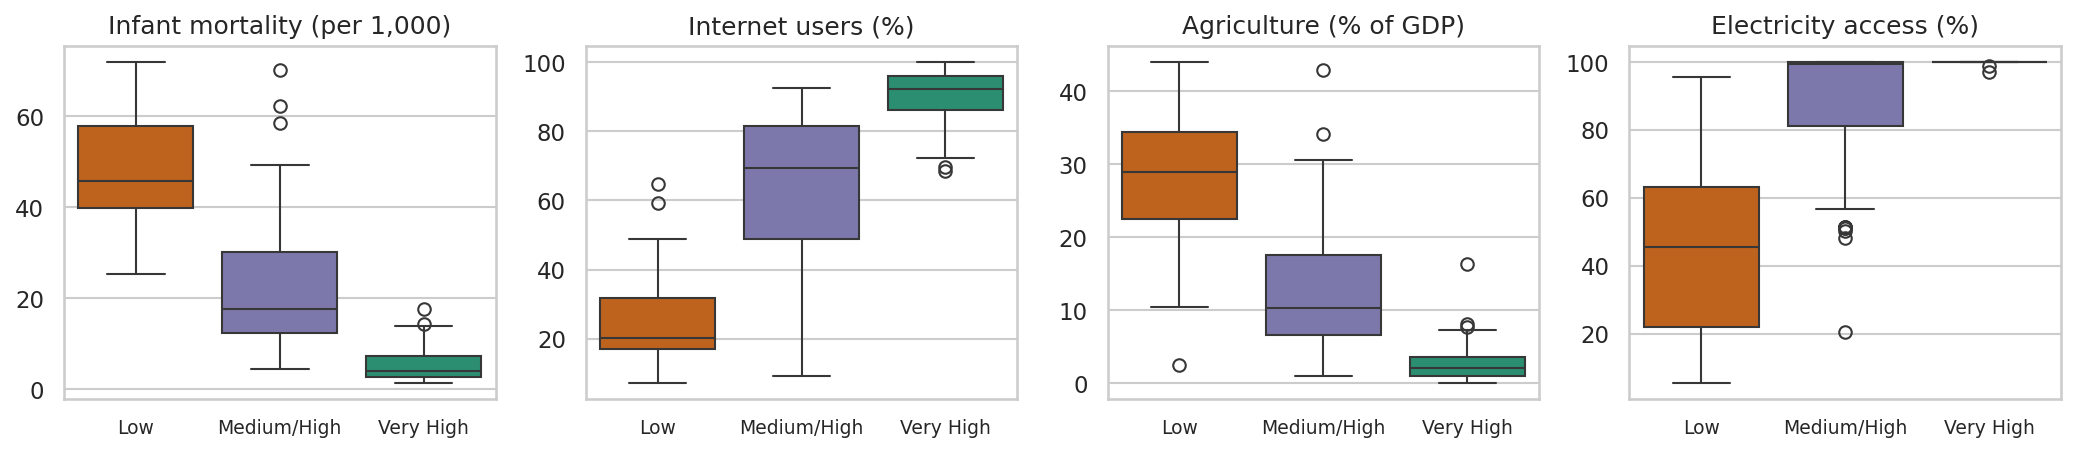
\includegraphics[width=\textwidth]{report_top_features_by_class.png}
  \caption{The four indicators that best separate the HDI classes (all 193 countries).}
  \label{fig:eda}
\end{figure}

\subsection{Imputation and model selection}

The imputation strategy made very little difference (Table~\ref{tab:imp}). All four options are within 0.015 CV
macro F1 of each other, while the standard deviation across folds is 0.05--0.09. Median and mean gave identical
results for logistic regression and the decision tree, likely because few values are imputed and the log
transform brings the mean and median close together. Missingness indicators gave a small, consistent gain for
logistic regression and the decision tree, which fits the EDA finding that missing data is more common in
low-HDI countries. We selected mean imputation with indicators (best average CV score). The indicators should be
read as a signal of data availability rather than of development itself.

\begin{table}[h]
\centering\small\setlength{\tabcolsep}{4pt}
\begin{minipage}[t]{0.37\textwidth}\vspace{0pt}\centering
\begin{tabular}{lccc}
\toprule
Imputation & LR & DT & RF \\
\midrule
Median & 0.857 & 0.848 & 0.909 \\
Mean & 0.857 & 0.848 & 0.917 \\
Median + ind. & 0.869 & 0.859 & 0.913 \\
Mean + ind. & \textbf{0.876} & \textbf{0.859} & \textbf{0.924} \\
\bottomrule
\end{tabular}
\captionof{table}{CV macro F1 for each imputation option (ind.\ = missingness indicators).}
\label{tab:imp}
\end{minipage}\hfill
\begin{minipage}[t]{0.61\textwidth}\vspace{0pt}\centering
\begin{tabular}{lcccc}
\toprule
 & CV F1 & \multicolumn{3}{c}{Test} \\
\cmidrule(lr){3-5}
Model & mean $\pm$ std & Acc. & Bal.\ acc. & Macro F1 \\
\midrule
Baseline & 0.216 $\pm$ 0.000 & 0.487 & 0.333 & 0.218 \\
Log.\ regression & 0.876 $\pm$ 0.066 & 0.821 & \textbf{0.730} & 0.726 \\
Decision tree & 0.859 $\pm$ 0.075 & 0.795 & 0.605 & 0.565 \\
Random forest & \textbf{0.924 $\pm$ 0.056} & \textbf{0.821} & 0.725 & \textbf{0.729} \\
\bottomrule
\end{tabular}
\captionof{table}{Model comparison: CV on the training set, and the held-out test set.}
\label{tab:models}
\end{minipage}
\end{table}

The random forest had the best CV score and was chosen as the final model (Table~\ref{tab:models}). The tuned
models were: logistic regression with $C=10$ and balanced class weights, a fully grown decision tree (depth 6, 13
leaves), and a random forest with maximum depth 5 and $\sqrt{p}$ features per split. On the validation set the
order was different (logistic regression 0.803, random forest 0.755, decision tree 0.717), but with 39 countries
these differences are within noise.

\subsection{PCA and feature sets}

After preprocessing there are 27 features. PC1 explains 23\% of the variance and 11 components are needed for
90\%, because each one-hot and indicator column adds its own direction. PC1 is a clear development axis, with
loadings on internet use (+0.46), infant mortality ($-$0.45), agriculture share ($-$0.43) and electricity (+0.41),
and the three classes are ordered along it. PC2 mostly captures the missingness indicators. Table~\ref{tab:abl}
shows that logistic regression with only \textbf{2 components} matches the full model (0.877 vs 0.876), so the
information that matters for the class is close to one-dimensional. The random forest, however, gets worse with
PCA (0.856 vs 0.924) because it works better when choosing among the original features. The final model
therefore does not use PCA.

\begin{table}[h]
\centering\small
\begin{tabular}{lccc}
\toprule
Feature set / variant & Logistic regression & Decision tree & Random forest \\
\midrule
Combined (numerical + region + sector) & 0.876 & 0.859 & \textbf{0.924} \\
Combined + PCA (tuned no.\ of components) & 0.877 ($k=2$) & 0.868 ($k=5$) & 0.856 ($k=3$) \\
Numerical only & 0.839 & 0.854 & 0.914 \\
Categorical only (region + sector) & 0.639 & 0.655 & 0.619 \\
Numerical + region & 0.876 & 0.851 & 0.923 \\
Numerical + DominantSector & 0.833 & 0.854 & 0.914 \\
\bottomrule
\end{tabular}
\caption{CV macro F1 (5-fold, training set) for PCA and for different feature sets. Baseline: 0.216.}
\label{tab:abl}
\end{table}

Most of the predictive signal comes from the numerical indicators. The categorical features on their own
(0.62--0.66) are far above the baseline but well below the indicators. Adding region helps logistic regression
the most (+0.037), while trees can already pick up regional patterns from the indicators. \texttt{DominantSector}
adds nothing, as expected for a feature that is 91\% one category and derived from shares already in the model.

\subsection{Test-set results and interpretation}

On the test set the random forest and logistic regression are effectively tied (macro F1 0.729 vs 0.726, both
82\% accuracy). Very High is classified almost perfectly (F1 $\approx$ 0.97) and Medium/High well (0.82), but Low
is hard: both models identify only 2 of the 5 Low countries (F1 = 0.40). As Figure~\ref{fig:cm} shows, both
only make mistakes between neighbouring classes. The fully grown decision tree misses every Low country and even
places two of them (Mali and Djibouti) in Very High. Its accuracy of
0.795 hides this, while its macro F1 of 0.565 shows it, which is why we did not rely on accuracy alone. The drop
from CV (0.92) to test (0.73) is mainly due to the Low class, where each of the 5 test countries is worth 20\% of
recall, together with the optimism of selecting the best of many CV configurations.

\begin{figure}[h]
  \centering
  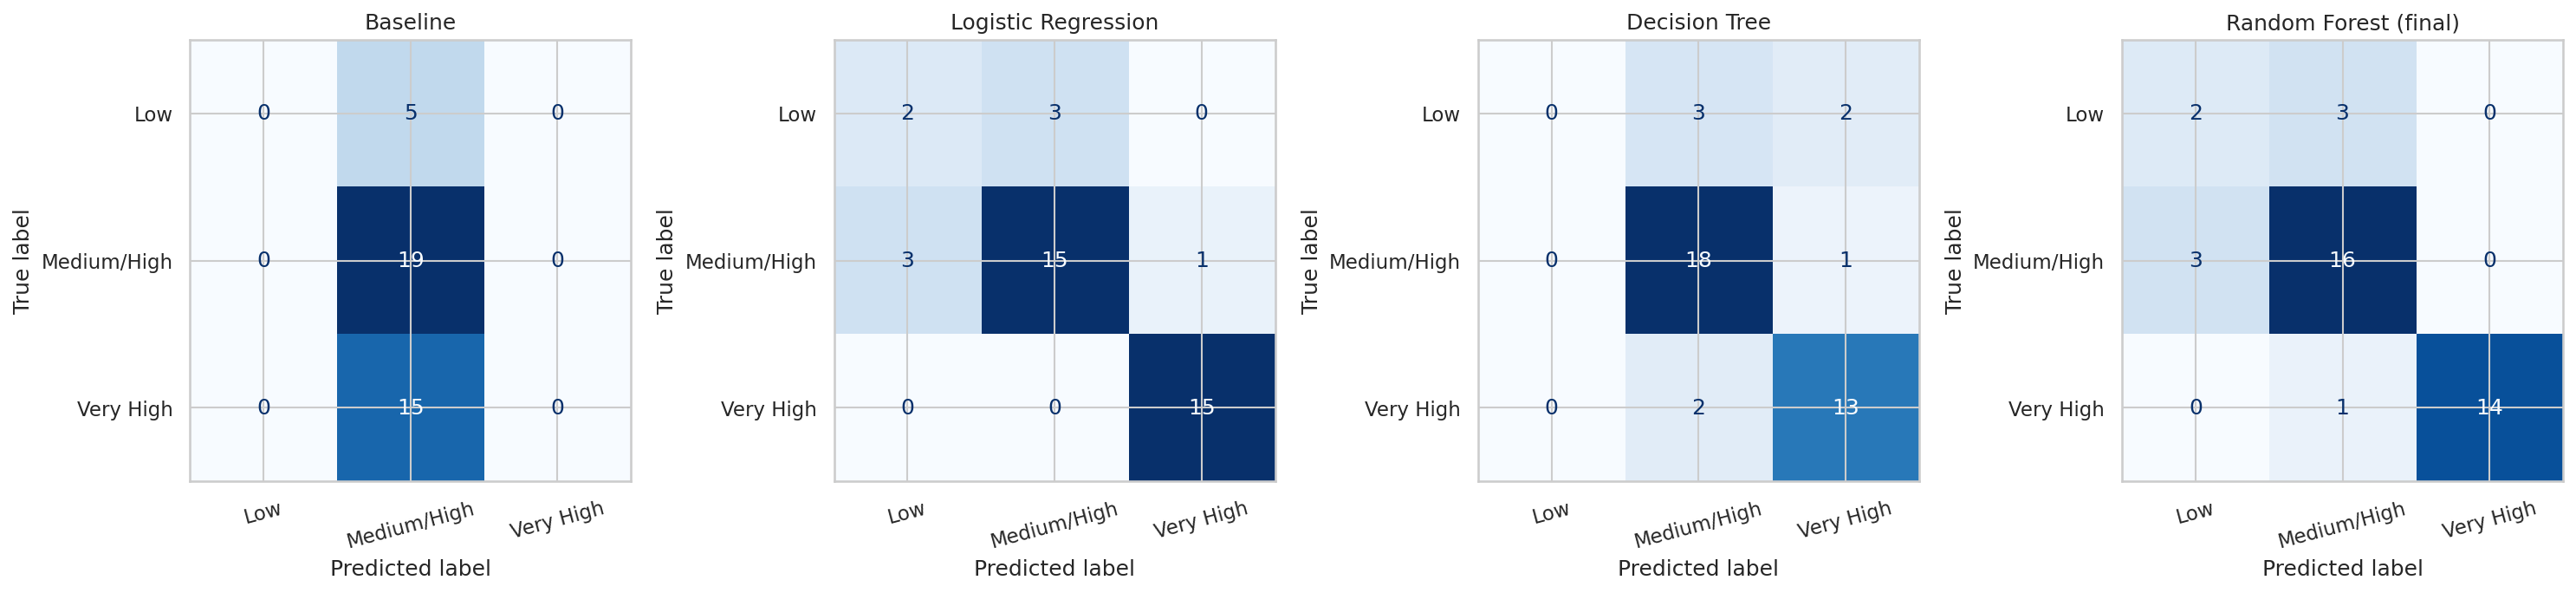
\includegraphics[width=\textwidth]{confusion_matrices_test.png}
  \caption{Confusion matrices on the 39 test countries.}
  \label{fig:cm}
\end{figure}

\begin{figure}[t]
  \centering
  \begin{minipage}[c]{0.5\textwidth}
    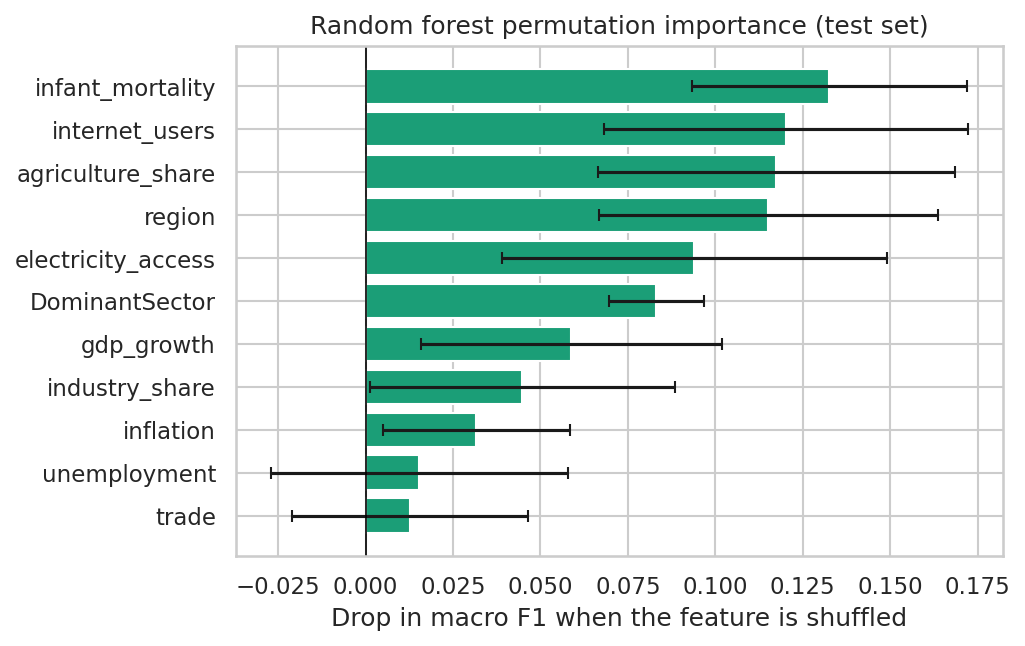
\includegraphics[width=\textwidth]{rf_permutation_importance.png}
  \end{minipage}\hfill
  \begin{minipage}[c]{0.46\textwidth}
    \caption{Random forest permutation importance on the test set: the drop in macro F1 when one feature is
    shuffled, averaged over 50 repeats (error bars show one standard deviation). The high value for
    \texttt{DominantSector} comes from only two test countries with a missing sector (see text).}
    \label{fig:imp}
  \end{minipage}
\end{figure}

The interpretation methods agree with each other and with the EDA. The largest logistic regression coefficients
belong to infant mortality (Low $+3.0$, Very High $-3.6$), internet use (Low $-3.4$, Very High $+2.9$) and
agriculture share (Low $+2.0$, Very High $-2.4$). Electricity access mainly separates Low from Medium/High
($-1.3$ vs $+1.3$), which matches its ceiling at 100\%. Because these features are strongly correlated, the
individual coefficients are not stable and only their overall direction should be trusted. Random forest
permutation importance (Figure~\ref{fig:imp}) puts infant mortality, internet use and agriculture share at the
top, with region almost level and then electricity access. Inflation, unemployment and trade contribute little. The importance of \texttt{DominantSector} is misleading: in the
test set only two countries are not ``Services'' (both have a missing sector), so its effect comes from those two
missing values. All seven random forest errors lie within 0.04 of a class boundary, for example Tanzania (0.555),
Gambia (0.524), Djibouti (0.513) and Sudan (0.511). The hard cut-offs turn small differences in the
score into wrong classes.

\subsection{Limitations and conclusion}

The main limitations are the small sample (193 countries is every country with an HDI, so the 39-country test set
gives a noisy estimate), the class imbalance (only 5 Low test countries), more missing data outside the Very High
class, and some predictors coming from 2020--2022 while the HDI is from 2023. Most importantly, the results
are associations. We cannot claim that changing an indicator would change a country's HDI, and infant
mortality is closely related to life expectancy, which is part of the HDI.

Overall, the random forest uses nine widely available indicators, region and dominant sector to place 82\% of the
test countries in the right HDI category, with all of its errors near the 0.550 and 0.800 cut-offs. Infant mortality,
internet use, agriculture share and electricity access are the most informative indicators. Since the class information is close to one-dimensional, predicting the HDI score
directly with regression would be a natural next step.

\begin{thebibliography}{9}\small
\setlength{\itemsep}{0pt}
\bibitem{undp} UNDP. \textit{Human Development Report 2025: composite indices time series} (HDR25).
\url{https://hdr.undp.org/data-center/documentation-and-downloads}. 
\bibitem{wdi} World Bank. \textit{World Development Indicators}, via the World Bank API v2.
\url{https://datatopics.worldbank.org/world-development-indicators/}. 
\end{thebibliography}

\end{document}
